\chapter{Implementing a Classifier for Isolated Signs}
\ifpdf
    \graphicspath{{Chapter2/Chapter2Figs/PNG/}{Chapter2/Chapter2Figs/PDF/}{Chapter2/Chapter2Figs/}}
\else
    \graphicspath{{Chapter2/Chapter2Figs/EPS/}{Chapter2/Chapter2Figs/}}
\fi
% ------------------------------------------------------------------------

\section{Implementing a Hidden Markov Model Class}
Our first task in implementing a classifier for signed languages was to implement a general purpose class \verb|DHMM| (figure:~\ref{fig:dhmmdiag}) which can be instantiated to model a Hidden Markov Model $\lambda = (A,B,\pi)$ by providing appropriate parameters. In this class we implemented solutions to the evaluation and training problems and provided methods for saving and loading the trained parameters. Extending the methods described in the previous section we taylored this implementation for use learning from a collection of data recorded from the Kinect Sensor. 
\subsection{Scaling}
In the previous section we introduced methods for solving the evaluation and re-estimation problems for Hidden Markov Models. These methods, whilst mathematically sound, introduced certain problems during implementation. In particular these solutions involve the products of a large number of probabilities, especially for long observation sequences, and as a consequence when implemented in C\# (which lacks arbitrary precision floats) can cause errors due to underflow. This problem is a common one in the implementation of Hidden Markov Models and to solve it we used the methods used by~\citet{rabiner1989tutorial} (and corrected by~\cite{rahimi2000}) and scaled the intermediate $\alpha$, $\beta$ and $\gamma$ variables to prevent underflow. To do this we normalize the $\alpha_t(i)$ by setting
\begin{align*}
\overline{\alpha}_1(i) = \alpha_1(i) \text{ for each $1\leq i\leq N$} 
\end{align*}
and inductively define for each $1 \leq t < T$
\begin{align*}
c_t &= \frac{1}{\sum_{i=1}^{N}\overline{\alpha}_t(i)}\\
\hat{\alpha}_t(i) &= c_t\overline{\alpha}_t(i)\text{ for each $i$}\\
\overline{\alpha}_{t+1}(i) &= \sum_{j=1}^{N}\hat{\alpha}_t(j)a_{ji}b_i(O_{t+1}) \text{ for each $i$}
\end{align*}
which prevents underflow in the intermediate calculation of the $\alpha$ variables. These scaled variables satisfy for each $1\leq i \leq N$ and $1 \leq t \leq T$
\begin{align*}
\hat{\alpha}_t(i) = c_1\dots c_t \alpha_t(i) 
\end{align*}
by induction on $t$~\citep{stamp2004revealing}. We then have that
\begin{align*}
1 = \sum_{i=1}^{N}\hat{\alpha}_{T}(i) &= c_1\dots c_{T}\sum_{i=1}^{N}\alpha_{T}(i)\\
&=c_1\dots c_{T}\mathbb{P}[\mathbf{O}|\lambda]
\end{align*}
and hence we can compute the log-probability of an observation sequence $\mathbf{O}$ by
\begin{equation*}
\log(\mathbb{P}[\mathbf{O}|\lambda]) = -\sum_{t=1}^{T}\log(c_t)
\end{equation*}
which allows us to determine probabilities which might have otherwise been lost due to underflow. 
We use the same scale factors on the $\beta$ variables by defining
\begin{align*}
\overline{\beta}_{T}(i) &= \beta_{T}(i) \text{ for each $1 \leq i \leq N$}
\end{align*}
and then inductively setting, for $1\leq t < T$ and $1 \leq i \leq N$
\begin{align*}
\hat{\beta}_{t}(i) &= c_t\overline{\beta}_t(i)\\
\overline{\beta}_{t}(i) &= \sum_{j=1}^{N}a_{ij}b_j(O_{t+1})\hat{\beta}_{t+1}(i)
\end{align*}
We then redefine the $\gamma$ variables for $1 \leq t < T$ and $1 \leq i,j \leq N$ as 
\begin{align*}
\gamma_t(i,j)&=\hat{\alpha}(i)a_{ij}b_j(O_{t+1})\hat{\beta}_{t+1}(j)\\
\gamma_t(i) &= \hat{\alpha}_t(i)\hat{\beta}_t(i)\frac{1}{c_t}
\end{align*}
Now if we use these variables in the re-estimation it is still the case that the the probability $\mathbb{P}[\mathbf{O}|\lambda]$ increases with each iteration~\citep{rabiner1989tutorial} and hence we can perform the iterative reestimation procedure for HMMs without introducing underflow errors.

\subsection{Training From Multiple Observation Sequences}
A second restriction of the training procedure presented in chapter 2 is that it restricts the training data of the HMM to be a single observation sequence. As we are going to train our HMMs on data which is derived from the Kinect Sensor data of a person performing a sign this is too great of a restriction. For example the way in which a person performs a sign will be unique each time and will differ between signers, and so to train a recogniser on a single observation sequence would not fully capture the range of movements which might be interpreted as that sign. Fortunately the reestimation procedure can be extended~\citep{li2000training,vano2010can, rabiner1989tutorial} to allow training from a set of multiple observation sequences $\mathcal{O} =\{\mathbf{O}_1, \dots, \mathbf{O}_{K}\}$ to maximise 
\begin{equation*}
\mathbb{P}[\mathcal{O}|\lambda] = \prod_{i=1}^{K}\mathbb{P}[\mathbf{O}_i|\lambda]
\end{equation*}
by computing for each $1 \leq i \leq K$ the set of scaled $\hat{\alpha}$, $\hat{\beta}$ and $\hat{\gamma}$ variables associated with the observation sequence $\mathbf{O}_i$ and the associated scales. Using these scaled variables we can reestimate the parameters of our HMM as
\begin{align*}
\overline{\pi_i} &= \frac{\sum_{k=1}^{K}\gamma^{(k)}_1(i)}{\sum_{j=1}^{N}\sum_{k=1}^{K}\gamma^{(k)}_1(j)}\\
\vspace{30mm}\\
\overline{a}_{ij} &= \frac{\sum_{k=1}^{K}\sum_{t=1}^{T_k-1}\hat{\alpha}^{(k)}_t(i) a_{ij} b_j(O^{(k)}_{t+1}) \hat{\beta}^{(k)}_{t+1}(j)}{\sum_{k=1}^{K}\sum_{t=1}^{T_k-1}\hat{\alpha}^{(k)}_t(i)\hat{\beta}^{(k)}_t(i)\frac{1}{c^{(k)}_t}}\\
\vspace{30mm}\\
\overline{b}_j(l) &= \frac{\sum_{k=1}^{K}\sum_{t \in \{1,\dots,T_k-1\}\text{ and $O_t = v_l$}}\hat{\alpha}^{(k)}_t(i)\hat{\beta}^{(k)}_t(i)\frac{1}{c^{(k)}_t}}{\sum_{k=1}^{K}\sum_{t=1}^{T_k}\hat{\alpha}^{(k)}_t(i)\hat{\beta}^{(k)}_t(i)\frac{1}{c^{(k)}_t}} \\
\end{align*}
and this will ensure that $\mathbb{P}[\mathcal{O}|\overline{\lambda}] \geq \mathbb{P}[\mathcal{O}|\lambda]$. Using this procedure we implemented the \verb|Reestimate| method of our \verb|DHMM| class.

\begin{figure}[h!]
        \centering
        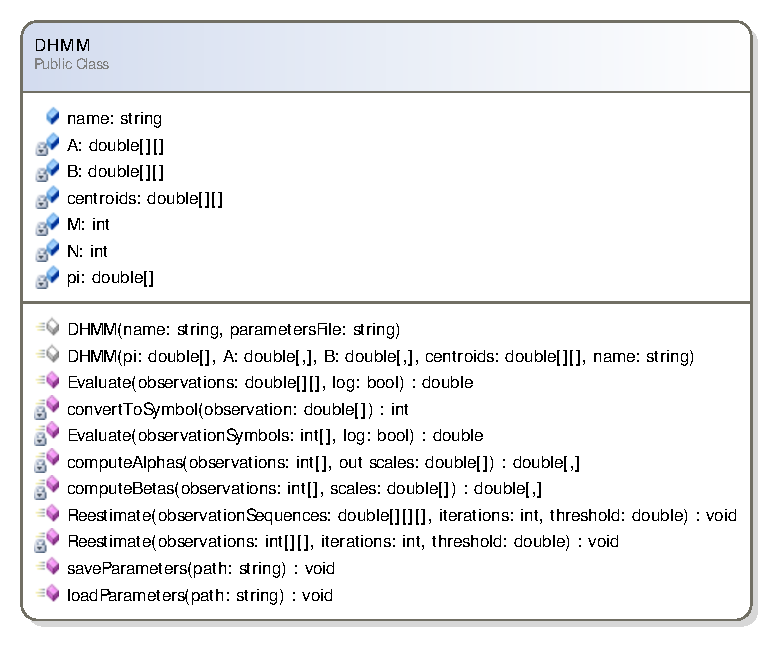
\includegraphics[width=0.8\textwidth]{ThesisFigs/DHMMDiag}
        \caption{A UML skeleton of the DHMM class}\label{fig:dhmmdiag}
\end{figure}

\subsection{Observation Vector Quantization}
In order to use discrete observation Hidden Markov Models for the problem of gesture recognition we must restrict the continuous observation space to a discrete set of observation symbols. As the ideal number of observation symbols was unknown we implemented a general purpose method for vector quantization.

To quantize the training data for a single discrete HMM instance we merged all of the points of all of the training data into a single 3D point cloud and partitioned this point cloud into $k$ clusters. To do this we implemented Lloyd's algorithm~\citep{lloyd1982least} to solve the k-means clustering problem (Figure:~\ref{fig:kmeans}). We then defined a translation from the continuous $\mathbb{R}^3$ observation space provided by the Kinect Sensor to a finite set of $k+1$ observations by assigning to each point the number of the cluster with the centroid closest (via Euclidean distance) to it, or $k+1$ if the distance from the point to each of the means exceeds twice the standard deviation of the cluster with the greatest variance. In fact, this quantization method will work just as well to translate arbitrary dimension continuous spaces to a finite observation set and hence offers us the opportunity to extend our training data sets to include not only spatial positions but other information as well, say velocity or positions relative to some fixed location.

Using this vector quantization method we were able to extend the \verb|Evaluate| and \verb|Reestimate| method of \verb|DHMM| to take as input streams of $(x,y,z)$ coordinates captured by the Kinect Sensor.

\begin{figure}[h!]
        \centering
        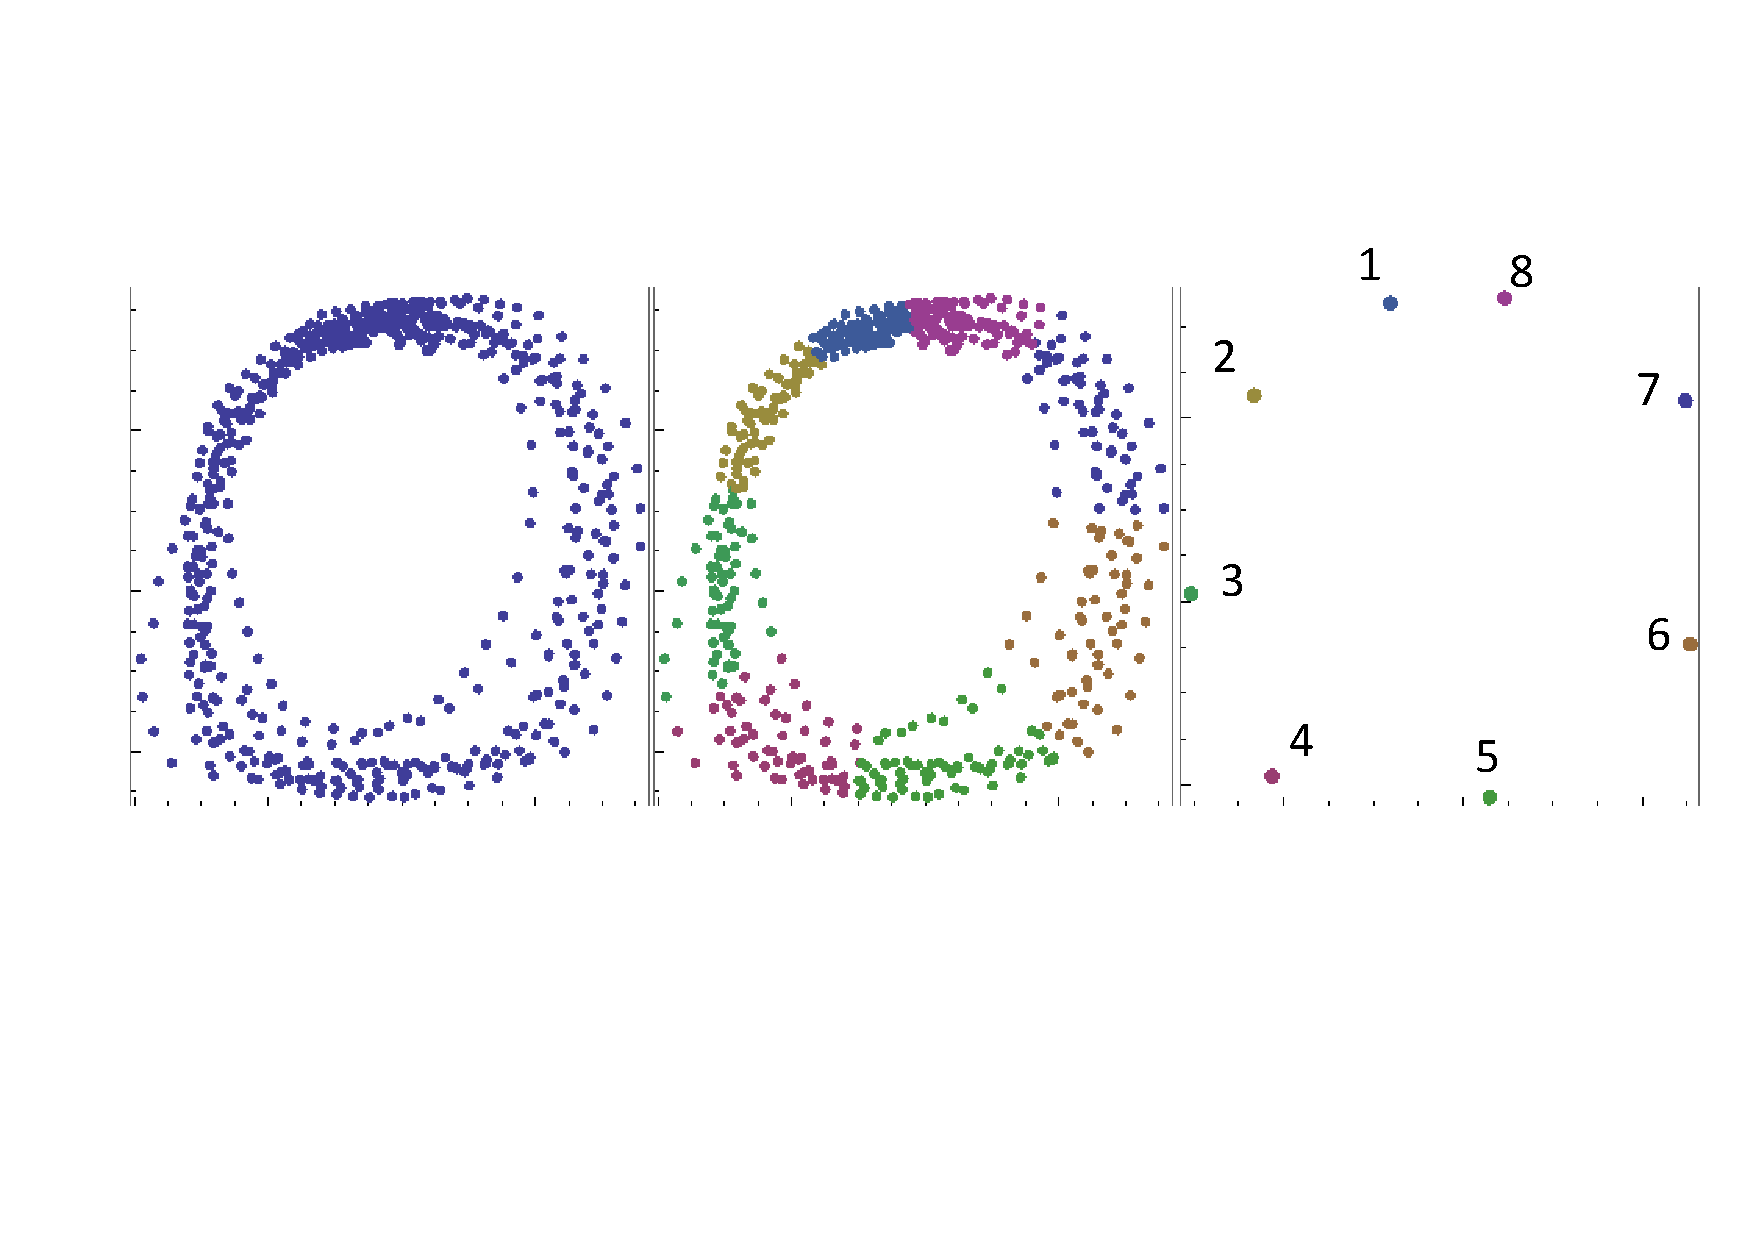
\includegraphics[width=0.9\textwidth]{ThesisFigs/ClusteringDiag}
        \caption{The K-Means method for vector quantization}\label{fig:kmeans}
\end{figure}

\section{Implementing the signModel class}
The main component of our sign classifier is a \verb|signModel| object which, when trained for a specific sign, can take a Kinect input stream and return the probability that the input stream corresponds to that sign. Our main problem was determining how to combine \verb|DHMM| objects to build an object which computes this probability by taking into account all of the information provided by the Kinect sensor.

One solution to this problem is to create an instance of \verb|DHMM| which takes as its input streams vectors of $(\mathbb{R}^3)^J$ where $J$ is the number of joints we choose to track. This method will allow us to detect signs using all of the joints tracked by the Kinect sensor however it does introduce two problems. The first is purely practical - the computations in the k-means clustering and training algorithms will become more and more expensive as the dimension of the observation vector grows and this will impact negatively on the performance of our sign recognition system.

The second issue is that this method ignores the prior knowledge we have about the joints of the body - that some are more dominant in the expression of a sign than others. For example, we know that the right hand is more dominant than the left and that both are more dominant than the elbows or shoulders. In fact the elbows and shoulders might be only worth considering when the hands alone cannot used to determine two different signs.

As such we should not let the importance of each joint be determined algorithmically and should specify these parameters with care. For this we create $J$ separate instances of \verb|DHMM|, each trained on a collection of observation sequences of a different joint. Then supposing we have trained a set of Hidden Markov Models $\Lambda = \{\lambda_1, \dots, \lambda_J\}$ for each joint, and have observation sequences $\mathbf{\Theta} = \{\mathbf{O}_1,\dots, \mathbf{O}_J\}$ which specify a stream for each joint over the course of one sign, we can compute a likelihood measure that this sequence corresponds to the sign used to train $\lambda_1, \dots, \lambda_J$ as a weighted sum
\begin{equation*}
L([\bm{\Theta} | \Lambda ]) = \sum_{j=1}^{J} c_j \log(\mathbb{P}[\mathbf{O}_j | \lambda_j])
\end{equation*}
where the weights $c_j$ are used to express the dominance of the $j^\text{th}$ joint in expressing a sign relative to the other joints. Note that this value no longer satisfies all of the properties of probabilities (or their logarithms) even if we restrict the constants in some way, however $L$ has one important property - that larger values correspond to more likely events. We choose to define $L$ in this way as it simplifies the computations in determining the likelihood that a given joint observation collection $\mathcal{O}$ corresponds to a given sign.

We implemented the class \verb|SignModel| (Figure:~\ref{fig:signModel}) to correspond to this definition of $\Lambda$. This class contains a collection of \verb|DHMM| objects with each corresponding to a joint of the skeleton provided by the Kinect Sensor, as well as a set of weightings corresponding to the $c_1, \dots , c_J$. Further there is a method \verb|trainModel| which trains an instance of \verb|DHMM| for each joint observation sequence set stored in the training folder. The \verb|signModel| class also contains a method to compute the likelihood that a given collection of joint observation sequences corresponds to this sign using the weighted sum of joints method described above.
\begin{figure}
        \centering
        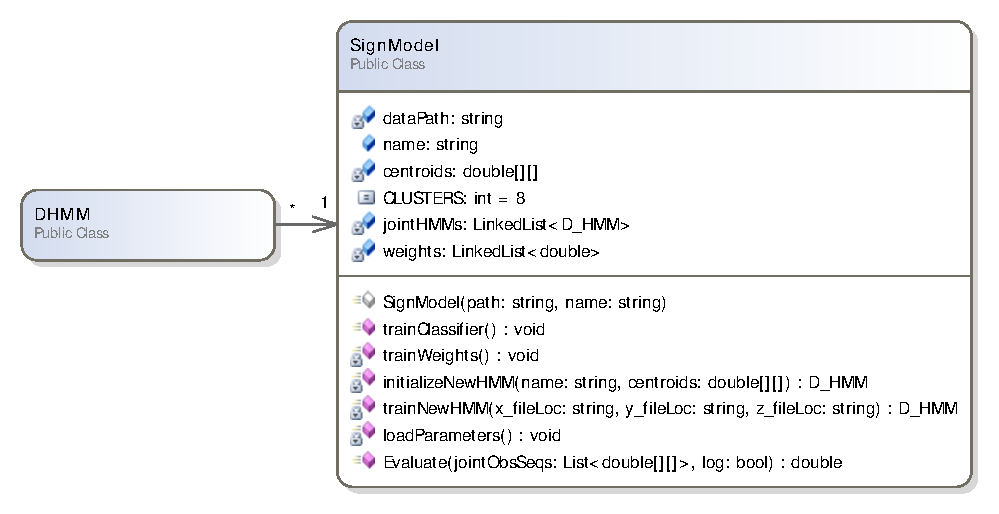
\includegraphics[width=1.03\textwidth]{ThesisFigs/signModelDiag}
        \caption{A UML diagram for the signModel class}\label{fig:signModel}
\end{figure}

\subsection{Determining the Weightings}
To ensure that the likelihood measures between signs are comparable we chose to use the same weighting constants for each sign model. Intuitively each constant $c_j$ corresponds to the importance of the joint $j$ in making a sign -- for example, the constants corresponding to the hands should be higher than those for the shoulders. In the absence of any research into the influence of the joints in signed languages we make the assumption that every movement a signer makes through the course of a sign is important. As such we determined that a greater variance of a given joint over the set of all training data implies that that joint conveys more information each sign. Hence, assuming $\mathcal{T}_j$ denotes the set of all observations of the joint $j$, we set
\begin{align*}
c_j := \sigma^2_j &= \frac{1}{\abs{\mathcal{T}_j}}\sum_{v \in \mathcal{T}_j} \norm{v - \mu_j}^2 &(\text{where } \mu_j = \frac{1}{\abs{\mathcal{T}_j}}\sum_{v \in\mathcal{T}_j}\norm{v})
\end{align*}
and then normalised the $c_j$ to satisfy
\begin{equation*}
\sum_{j \in J} c_j = 1
\end{equation*}
We decided that if a joint $j$ has $c_j < 0.05$ then it is unlikely  to impact the overall decision about which sign has been observed and that the calculation of $\mathbb{P}[\mathbf{O}_j | \lambda_j]$ would be a waste of computational resources. As such we decided to set $c_j = 0$ for these joints and forgoe the unnecessary calculations. Using this method we chose to ignore the head, chest and lower body joints provided by the Kinect sensor.

\subsection{Determining The Initial Topology and Parameters}
As our training method utilises a local search to improve our parameterisation its effectiveness will greatly depend on how we initialise our Hidden Markov Models. If the initial parameterisation is poor then even with a large training set we may fail to find a parameterisation which allows us to recognise signs with high accuracy.

It has been shown that the topology of the underlying Markov Chain can greatly impact the effectiveness of a HMM for a given pattern recognition task~\citep{rabiner1989tutorial, jelinek1998statistical}. The two most common types of HMM (See figure ~\ref{fig:mctop}) are the \emph{ergodic model}, in which each state can transition to any other state in a finite number of steps and the \emph{left-right model} or Bakis model~\citep{bakis1976continuous} in which the state sequence is (non-strictly) increasing. The left-right model can be viewed as modelling a signal which changes through time, with each transition representing a movement forward in time. For that reason it is more suitable for modelling gestures or speech than other Markov Chain topologies and is the topology we chose for our Hidden Markov Models.

A left-right topology Markov chain is characterized by an upper triangular stochastic matrix $A$. We can further restrict our model to only allow jumps from a state $i$ to states $i \leq j \leq i+\Delta$ for some $\Delta$. This restriction can prevent the model being pushed, through re-parameterisation, into a trivial Markov chain which remains at the final state $N$ at all times. This can be seen as imposing a restriction on the velocity we can expect a signer's hand to move at - not allowing him to pass by too many states in quick succession.

\begin{figure} [t]
        \centering
        \begin{subfigure}[b]{0.45\textwidth}
                \centering
                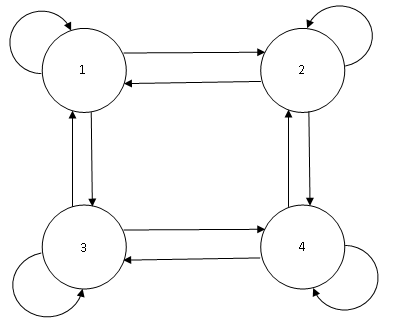
\includegraphics[width=1.0\textwidth]{ThesisFigs/erdogicMC}
                \caption{An Ergodic Markov Chain}
                \label{fig:unclust}
        \end{subfigure} \\
        \begin{subfigure}[b]{0.5\textwidth}
                \centering
                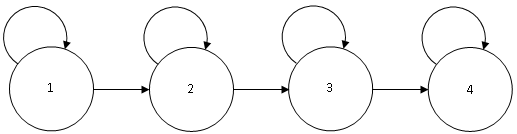
\includegraphics[width=1.0\textwidth]{ThesisFigs/del1LRMC}
                \caption{A $\Delta = 1$ Left-Right Markov Chain}
                \label{fig:clust}
        \end{subfigure}
	   \begin{subfigure}[b]{0.5\textwidth}
                \centering
                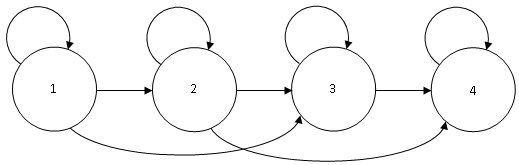
\includegraphics[width=1.0\textwidth]{ThesisFigs/del2LRMC}
                \caption{A $\Delta = 2$ Left-Right Markov Chain}
                \label{fig:clust}
        \end{subfigure}
        \caption{Different Markov Chain Topologies}\label{fig:mctop}
\end{figure}

As such we choose to intialize the HMMs in the \verb|signModel| class as left-right models restricted to $\Delta = 1$ and initialise the stochastic matrix with form
\begin{equation*}
A =
 \begin{pmatrix}
  a_{11} & a_{12} & 0 & \cdots & 0 \\
  0 & a_{22} & a_{23} &\cdots & 0 \\
  \vdots  & \vdots  & \vdots & \ddots & \vdots  \\
  0 & 0 & \cdots & a_{(n-1)(n-1)}& a_{(n-1)n} \\
  0 & 0 & \cdots & 0& 1
 \end{pmatrix}
\end{equation*}
and define $\pi = [1,0, \dots, 0]$. Clearly if we initialise the non-zero $a_{ij}$ of A deterministically then we restrict ourselves to single outcome from the re-estimation procedure regardless of how many times we retry it, as such we choose to introduce some stochasticity by setting
\begin{align*}
&a_{ii} = 0.5 - r &a_{i(i+1)} = 0.5 + r
\end{align*}
 for some $r$ chosen uniformly from the interval $[-0.3, +0.3]$. This interval is chosen to ensure that none of the links are set too weakly causing the forward transitions to be broken during re-estimation.

As we expect the system to differentiate a large number of signs it would be a major task to tailor the initialisations of each Hidden Markov Model to the sign it is expected to recognise. Hence, we choose to use the same initial estimation procedure for each HMM and do not make any inferences about the structure of the emissions matrix $B$ given the sign it is expected to model. We initialise $B$ almost uniformly with
\begin{align*}
&b_{ij} = 1/M + r_{ij} &\text{for each $1\leq i \leq N$ and $1 \leq j \leq M$}
\end{align*}
where each $r_{ij}$ is some small random number and subject to the condition that the matrix $B$ remains stochastic.

The benefit of introducing stochasticity into the initial parameter estimations is that if the re-estimation procedure does not produce a sufficiently good parameterisation we can re-initialise our HMM and try again. That is to say we may use the forward-backward algorithm as part of a random restart hill climbing algorithm~\citep{russell1995artificial} to increase the chances that we will find a good parameterisation for the model.

\section{Building a Sign Classifier}
A \verb|signModel| object, when trained using suitable set of training data from a single sign, allows us to evaluate how likely a new observation sequence is to be an instance of the sign used to train the model. Hence if we have a trained \verb|signModel| instance $m_s$ for each sign $s$ in some dictionary $D$ and a collection of joint observation sequences $\bm{\Theta} = \{\mathbf{O}_1, \dots, \mathbf{O}_J\}$ read from the Kinect Sensor then we can determine which sign model was most likely to have generated $\mathcal{O}$ as
\begin{equation*}
m = \text{argmax}_{s \in D}\{ L[\mathcal{O}|m_s]  \}
\end{equation*}
where the value $L[\mathcal{O}|m_s]$ is computed by the \verb|Evaluate| method of the \verb|signModel| object. Then if $L[\mathcal{O}|m]$ is sufficiently large, say greater than some threshold $\tau$, we can conclude that $\mathcal{O}$ corresponds to the sign used to train $m$. 

We implemented this means of determining a signs as the class \verb|signClassifier| (Figure:~\ref{fig:scuml}) which contains for each sign a trained \verb|signModel| object and a method \verb|getSign| which performs the above calculation.
\begin{figure}[t]
        \centering
        \includegraphics[width=1.04\textwidth]{ThesisFigs/classDiag}
        \caption{The signClassifier in UML}\label{fig:scuml}
\end{figure}

A trained instance of \verb|signClassifier| forms the basis of SignAlign and provides a means of recognising signs using the Kinect Sensor as input. We implemented the \verb|buildClassifier| method to search for any parameterisations for \verb|signModels| on disk and load them and then to search for any new training sets and create new \verb|signModel| instances from them (saving their parameters to disk). As such the SignAlign dictionary can be extended by simply providing more training data without the need to retrain the rest of the model. This is a particularly desirable feature as a full re-estimation can take considerable time for a large dictionary and it would be inconvenient to perform each time the dictionary is expanded.

The \verb|signClassifier| and \verb|signModel| classes contain a number of contants which we have not yet given a specified value, for example $M$ the number of observation symbols or the acceptance threshold $\tau$ for detecting a sign. There is no \emph{a priori} reason we should choose any particular value for these signs and hence chose to determine them through experimentation (Chapter 5). Before this was possible we were required to build a catalogue of training data and test cases by recording Kinect sensor streams.
% ------------------------------------------------------------------------

%%% Local Variables: 
%%% mode: latex
%%% TeX-master: "../thesis"
%%% End: 
